\documentclass[12pt]{report}

\usepackage{amsmath,amssymb,amsfonts}
\usepackage{listings}
\usepackage{graphicx}
\usepackage{hyperref}
\usepackage{fancyhdr}
\usepackage{color}
\usepackage{lettrine}
\usepackage{textcomp}
\usepackage[utf8]{inputenc}
\usepackage[toc,page]{appendix}
\usepackage{courier}

\usepackage[margin=2cm]{geometry}

\definecolor{dgrey}{rgb}{0.3,0.3,0.3}
\definecolor{dyellow}{rgb}{0.6,0.6,0.0}
\definecolor{gblue}{rgb}{0.35,0.35,0.6}

\hypersetup{
	colorlinks=true,
	linktoc=all,
	linkcolor=gblue,
	citecolor=dyellow,
}

\lstset{basicstyle=\ttfamily\footnotesize, frame=single,
breaklines=true,showstringspaces=false,numbers=left}

\title{ECSE 323 - Digital System Design\\After Action Report - The Dealer Finite State Machine}
\author{Harley Wiltzer (260690006)\\Spiros-Daniel Mavroidakos (260689391)}
\date{March 30, 2017}

\begin{document}
\pagenumbering{gobble}
\maketitle
\newpage
\pagestyle{fancy}
\fancyhf{}
\rhead{Harley Wiltzer (260690006), Spiros-Daniel Mavroidakos (260689391) - Vandelay Industries}
\pagenumbering{arabic}
\tableofcontents

\part{A Pleasant Preamble}
\label{s:preamble}
\lettrine{S}ometimes in life one may be presented with situations that make him rethink his beliefs and
question who, in fact, he really is. It is moments like such that actually define an individual
\textit{ad postremum}. Of course, it is up to the individual in question to \textit{realize} that he shall be
withdrawing cathexis from the myriad objects of empirical reality around him if enlightenment should
be obtained. People that occasionally experience this enlightenment are called patricians. Those who
continuously experience this enlightenment are called Engineers.\\\\
Consider the infamous game of Blackjack. Some may enjoy this game as a nice way to pass the time,
others may be violently obsessed with it. Regardless of who is playing, the game can only be played
reliably when players understand and follow the rules and when a credible dealer is present.
Naturally, the players are needed for the game to be played, and of course the game is only really
\textit{being played} when the rules are followed. The presence of the dealer, however, is far more
interesting than what the uninformed reader may believe.\\\\
Some say the dealer's job is to deal the cards, but that is a vast and decadent oversimplification.
Sure, the dealer \textit{should} deal the cards (at the appropriate times, that is), but the dealer
is also responsible for establishing structure and ensuring that the game does not get out of hand.
In fact, the rules of the game themselves have their strings pulled by the dealer. \\But some dealers
do not follow the rules.\\\\
It is no longer news that the goal of these laboratory sessions is to build a \textit{crazy eights}
game, and not a Blackjack game. Although the rules of the two games are different, both take on the
rules-dealer paradigm of gameplay. The layman, and even the patrician, may focus on the rules of the
game principally. However, as Engineers, the main focus of this laboratory was to create not just a
functional dealer, but a reliable, ethical, and ultimately compliant dealer. As shown later in this
report, this was successfully accomplished due to the design of a clever \textit{finite state
machine}, a construct that has also been used in the design of underwhelming robots.\\\\
In the interest of moral behavior, it would be unethical to display the accomplishments of this
laboratory session without giving due credit to the Altera Quartus II and Modelsim software, whose
magical functionalities allow such complex designs to be mapped onto an FPGA. Also, with such great
text editing accomodations and incredible timing simulation tools, the development of this system
was dream-like.\\\\
At this stage, the reader is invited to explore the remainder of this report, which will go through
in a (hopefully) simple and organized manner the discoveries made during this laboratory session.
Beyond that, this report will discuss \textit{how} these discoveries were made, and how they were
reinforced, so the reader may gain intuition on developing state of the art digital systems.\\\\
Please enjoy the remainder of this report, and try to learn something from it. Much is to be gained
by grasping the concepts of the rules-dealer paradigm, as they apply to more in life than simply
digital systems and card games. To conclude this pleasant preamble, the reader is encouraged to,
above all, \textit{have fun} with this report, and better yet, to have fun with life. Finally, it is
important to remember that while by law a man is guilty for violating the rules, in ethics a man is
guilty merely by \textit{considering} such violation. Be careful, be wise, and Baba Booey to all.

\part{The Dealer Circuit}

\chapter*{Introduction}
\addcontentsline{toc}{chapter}{Introduction}
As foreshadowed in the \hyperref[s:preamble]{pleasant preamble} above, having a loyal, dependable
dealer will be crucial to the reliable functionality of the crazy eights system. Without such a
dealer, the \textit{rules} of the game \textit{may not} be followed, causing complete and utter
pandemonium, ultimately resulting in a rather atrocious crazy eights game.\\\\
Therefore, it would benefit the system to create a robust \textit{finite state machine}, a machine
of a finite number of states. The system was reduced to a machine of 4 states (where $4 < \infty$
holds), representing the state which waits for the previous request to end (denoted by A), the state
which waits for the next request to \textit{be} sent (denoted by B), the state which generates
random numbers, so as to deal the cards (denoted by C), and finally, the state that activates a
stack (or more accurately, a bi-directional Jenga tower) circuit (denoted by D). \\\\
All of the cleverness and power that has been teased above was encompassed by a circuit that has
since been named the \texttt{g07\_dealerFSM}. A more detailed insight to the design of the finite
state machine and the \texttt{g07\_dealerFSM} follows below, and is complemented by thoughtful
pictorial support for easier understanding.

\chapter*{Circuit Description}
\addcontentsline{toc}{chapter}{Circuit Description}

\begin{figure}[h]
	\begin{center}
		\caption{Pin-out diagram of the \texttt{g07\_dealerFSM} circuit}
		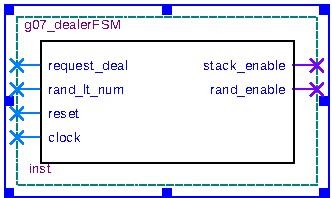
\includegraphics[scale=1.3]{dealer_symb}
	\end{center}
\end{figure}

Above is a pin-out diagram of the miraculous \texttt{g07\_dealerFSM} circuit, showcasing its input
and output ports. A more detailed description of these ports will be given below.

\section*{Description of ports}
\addcontentsline{toc}{section}{Description of ports}
\subsection*{request\_deal}
The \texttt{request\_deal} input bit is activated when the system requests that the dealer should
deal a card.
\subsection*{rand\_lt\_num}
The \texttt{rand\_lt\_num} input bit is controlled by an external circuit that is high when a random
number has a value that is less than the BJT's \texttt{NUM} output that the dealer is associated
with. This allows the dealer to tell whether it should keep generating random numbers (in state C),
or move on.
\subsection*{reset}
The \texttt{reset} input bit causes the finite state machine to be reset to its initial state when
\texttt{reset} is high. It is asynchronous.
\subsection*{stack\_enable}
The \texttt{stack\_enable} output bit is active when a valid random number has been generated in the
proper state. It is used to enable the BJT associated with the dealer to pop a card.
\subsection*{rand\_enable}
The \texttt{rand\_enable} output bit is active after \texttt{request\_deal} has been asserted anew,
and enables a random number generator to generate random numbers until \texttt{rand\_lt\_num} is
high.

\end{document}
